\chapter{LaTeX Basics}\label{app:latex}

\LaTeX\ is a software system which requires plain text and compiles it into a formatted document subsequently. This means the user merely has to pay attention to the structure and create chapters, sections, subsections, subsubsections, paragraphs and subparagraphs. Commands start with a backslash ($\backslash$) and the percentage sign (\%) or shortcut Ctrl + T is used to create a comment. %comment

\section{Literature}
Literature references should be inserted into the \texttt{references.bib} file. They can be exported in the BibTeX format from most online sources, however, it should be paid attention that the information is complete and in the same format as the other sources. Subsequently the source can be referenced with the \texttt{$\backslash$cite} command.

\section{Equations}

One large advantage is that equations can be inserted easily, as in~\eqref{eq:1}.  These have to be written in a specific math-environment. It is most commonly created by using \texttt{$\backslash$begin\{equation\}} and \texttt{$\backslash$end\{equation\}} for a single equation, \texttt{$\backslash$begin\{align\}} and \texttt{$\backslash$end\{align\}} for multiple equations, and dollar signs for a \$$mathematical\ expression$\$ in the text.

\begin{equation}
\alpha = \frac{\beta^2}{\gamma}\label{eq:1}
\end{equation}

\section{References}
Using the command \texttt{$\backslash$label} nearly everything can be labeled in the document, from chapters and sections to equations, figures or tables. \texttt{$\backslash$ref} creates a reference in the text, such as for figure~\ref{fig:graph}. Equations are usually referenced using \texttt{$\backslash$eqref}.

\section{Floats}
Figures or tables are referred to as floats because they cannot be broken over a page. They are automatically positioned depending on the placement in the text and the specifier in the square brackets, i.e. \texttt{h, t, b, p} (referring to here, top, bottom, page, respectively). The environment is again created using the \texttt{$\backslash$begin} and \texttt{$\backslash$end} commands. Figures should be inserted as vector graphics (\texttt{.eps}) if suitable. Graphs can also be inserted using the package \texttt{pstricks}.
Captions for figures are placed below the float, the ones for tables above. Furthermore, a short version of the caption can be inserted in the angular brackets and will appear in the list of figures/tables.


\begin{figure}[t]
\centering
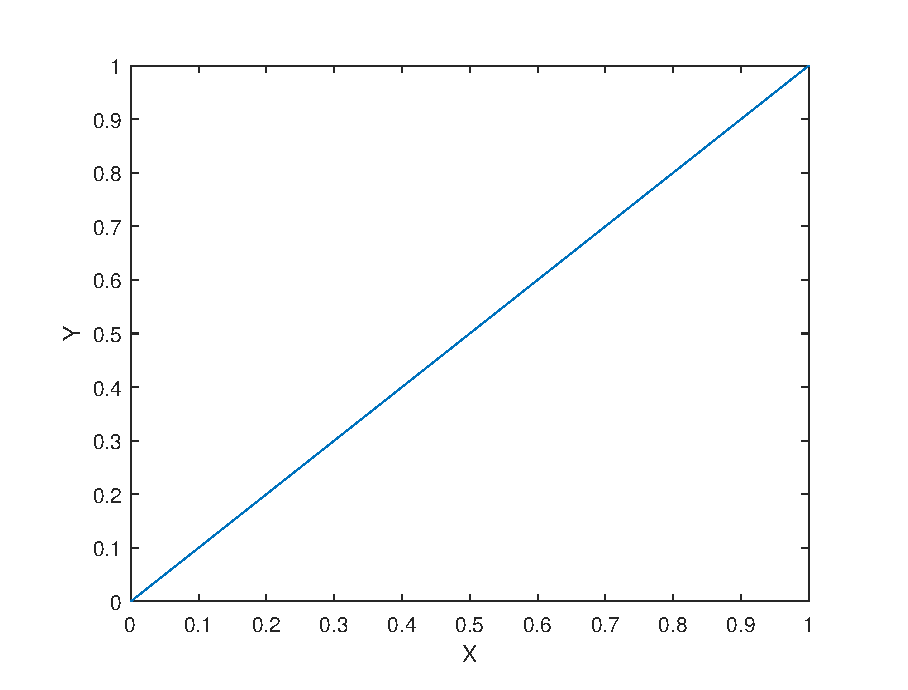
\includegraphics[width=0.75\textwidth]{figures/graph.eps}
\caption[Graph]{Insert figures as .eps-files if suitable.}
\label{fig:graph}
\end{figure}

\begin{table}[t]
\centering
\caption[Table]{Table}\label{tab:table}
\begin{tabular}{c|cc}
\hline
& System 1 & System 2\\\hline
Data 1 & 0.1 & 0.2\\
Data 2 & 0.3 & 0.4\\\hline
\end{tabular}
\end{table}


\section{Further information}
For further information on LaTeX, such as commands for mathematical symbols or conventions on cross-referencing consult the documentations at \url{https://en.wikibooks.org/wiki/LaTeX} and \url{https://overleaf.com/learn}. Most of the issues regarding certain kinds of formatting in LaTeX have also been addressed in one of the multiple LaTeX-forums online.